\section{Results}
\label{Results}

\subsection{Ionization State}

%Results:
%Log_Ionized_vs_Redshift.png

In the literature, people working on the epoch of reionization use terms such as ionized or neutral region to inidicate places where Hydrogen is mainly ionized or neutral, but what is missing is the degree to which that statement is true.  Figure \ref{Log_Ionized_vs_Redshift}. shows that there are different levels of ionization.  This graph quantifies the ambiguities of what ionized means.  We now can tell at any given redshift, how much of the volume is ionized to what degree.  The curve labelled "10\%" shows the volume fraction of the universe ionized to 10\%, meaning having MORE than 1 ionized Hydrogen particle per 10 Hydrogen particles.  The curve labelled "1e-3" means having LESS than 1 neutral Hydrogen particle per 10$^3$ Hydrogen particles, and "1e-5" means having LESS than 1 neutral Hydrogen particle per 10$^5$ Hydrogen particles.  For example, we can tell that when 10\% of the universe's volume is ionized to 10\%, this occurs around a redshift of 8.7 (estimates are from simple linear interpolation of the available output data at certain time intervals).  And if we use another degree of ionization, we can say 10\% of the universe's volume is ionized to 1e-5 around a redshift of 7.7.  The numerical values may be cumbersome to read, so we will use "Ionized" to designate the 10\%, "Well Ionized" to designate the 1e-3, and "Fully Ionized" to designate the 1e-5 ionization levels for the rest of the paper.  This graph ultimately shows that more of the universe becomes more highly ionized as redshift decreases.

\begin{figure}
  \includegraphics[width=0.5\textwidth]{bLog_Ionized_vs_Redshift.eps}
  \caption{\footnotesize Ionized Volume Fraction for different degrees of ionization.  
    The solid line is 10\% (Ionized), the dash line is 1e-3 (Well Ionized), and the dash-dot line is 1e-5 (Fully Ionized)}
  \label{Log_Ionized_vs_Redshift}
\end{figure}

% threshold 1e-5 for z=6 for that one point

\subsection{Clumping Factor Calculation}

%Clumping_vs_Redshift.png
A widely used indicator of recobination, hence the photon requirement for ionizing the universe during the epoch of reionization, is the H {\footnotesize II} clumping factor \citep{ValageasSilk1999b}.  
\begin{equation}
\label{ClumpingFactor}
C = \frac{<n>^2}{<n^2>}
\end{equation}
In pure N-body simulations, people usually assume that the baryons follow dark matter, and for non-radiation processed simulations, assume that the gas is completely ionized when calculating the clumping factor\citep{LoebBarkana2001}.  So essentially they are just using the dark matter clumping factor in place of the H {\footnotesize II} clumping factor (using the dark matter density in place of n in Equation \ref{ClumpingFactor}).  Figure \ref{Clumping_vs_Redshift}.  shows that there is a range of values for the clumping factor calculated from different assumptions.  The "H {\footnotesize II}" thin dash curve is the clumping factor vs. redshift calculated from H {\footnotesize II}.  The thick dash curve labelled "Dens" is calculated from baryon density.  The thick solid curve labelled "DM" is calculated from dark matter. The curves with the prefix of "t" means that it was calculated using  only cells that satisfy a set threshold. The first threshold applied picks cells with dark matter density below 100 times the global mean dark matter density value.  The curve with two t's has, in addition to the dark matter density threshold, a Hydrogen ionization fraction above 10\%.  If we were to assume that the baryons traces dark matter, then the clumping factor would follow the curve labeled "DM", because that is how clumpy the dark matter evolve.  If we were to forgo that assumption, then to calculated the baryon clumping factor, assuming that all the gas is ionized, we would be following the curve labeled "Dens".  And if we were to not assume that all the gas is ionized and calculate the clumping factor for H {\footnotesize II} directly, we would follow the curve labeled "H {\footnotesize II}".  In their paper, \citep{RaicevicTheuns2011} argued that if we were to calculate the local clumping factor while thresholding the region that is virialized, we would get a better estimate of the recombination from clumping factor.  So if we were to apply such a threshold, looking at the single t prefix curve, we see how the different curves behave compared to their counter part.  We follow the same train of thought and consider what will happen to the clumping factor if we only look at how clumpy the gas is in the Ionized region of the volume.  That reasoning gives the ttH {\footnotesize II} curve.  One thing to note here is that, when the double threhshold is applied, we are calculating the clumping factor of spatially disjoint regions.  However, all this thresholding just futher highlights the fact that one can get different clumping factors depending on the assumptions made about the baryonic matter and the radiation field.

\begin{figure}
\label{Clumping_vs_Redshift}
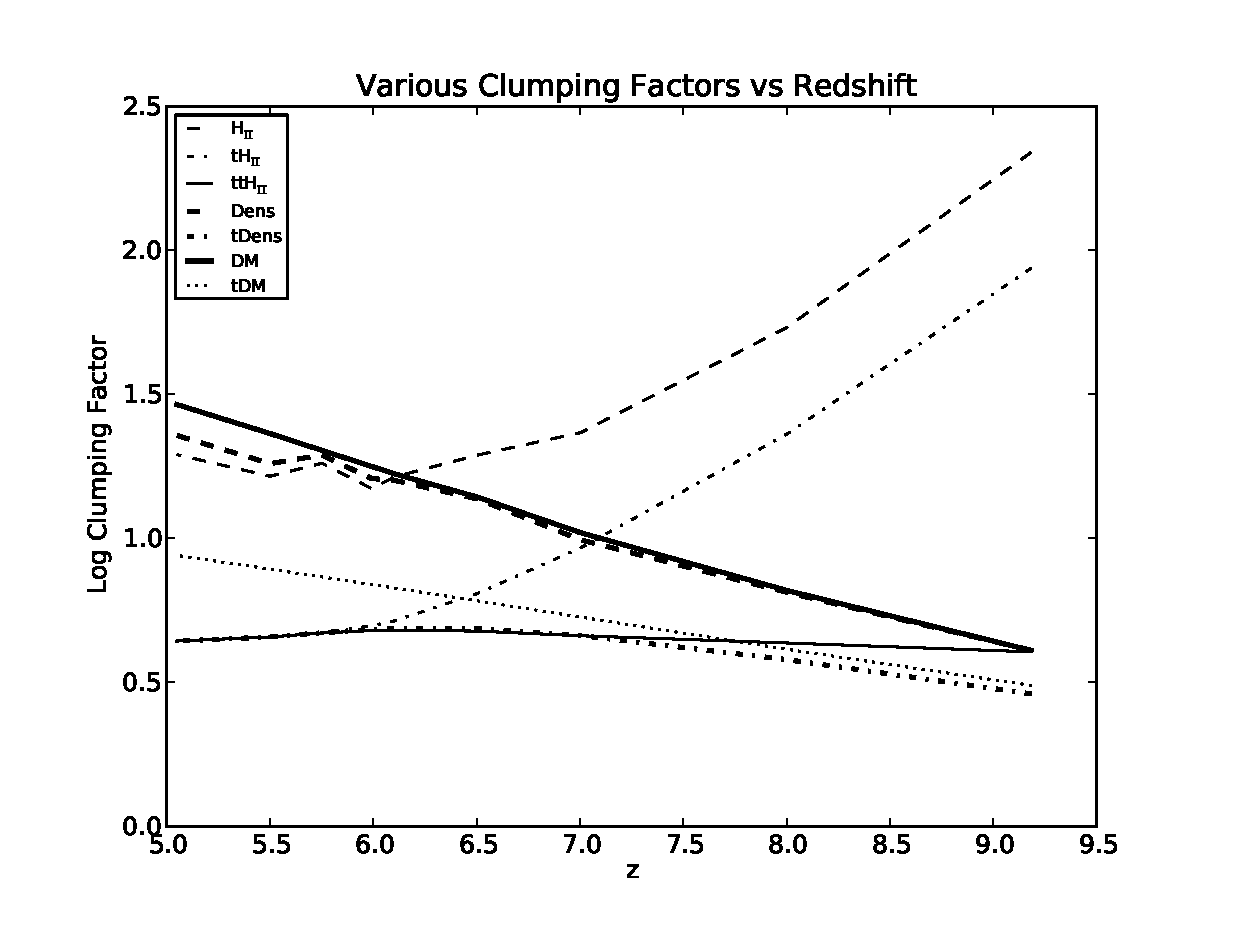
\includegraphics[width=0.5\textwidth]{bClumping_vs_Redshift.eps}
\caption[cap]{\footnotesize
	\begin{inparaenum}
		\item H {\footnotesize II} clumping factor calculated from HII\_Density field in Enzo.
		\item tH {\footnotesize II} clumping factor from HII\_Density with first threshold applied.
		\item ttH {\footnotesize II} clumping factor from HII\_Density with second threshold applied.
		\item Dens clumping factor from Density field (Baryon) in Enzo.
		\item tDens clumping factor from Density with first threshold applied.
		\item DM clumping factor from Dark\_Matter\_Density field in Enzo.
		\item tDM clumping factor from Dark\_Matter\_Density with first threshold applied.
	\end{inparaenum}
	First threshold excludes cells that have Dark\_Matter\_Density that are over 100 times the global mean Dark\_Matter\_Density.  Second threshold excludes cells below 10\% ionized.}
\end{figure}

% explain how the volume is disjoint when thresholding

\subsection{Photons vs. Recombinations}

%photon_to_ionize.png
Now let us explore the connection between clumping factor and the epoch of reionization.
\begin{equation}
\label{Ndot}
\dot{N}_{ion}(z)=10^{51.2}s^{-1}Mpc^{-3}\left(\frac{C}{30}\right)\left(\frac{\Omega_b h^2}{0.02}\right)^{2}\left(\frac{1+z}{6}\right)^{3}
\end{equation}
Equation \ref{Ndot}. is used in the literature to estimate the photon rate density, the photons produced per second per Mpc$^3$ required to keep the universe ionized \citep{FanCarilliKeating2006}.  Using the different clumping factors in Figure \ref{Clumping_vs_Redshift}. in place of C in Equation \ref{Ndot} we get the various curves on Figure \ref{Photon_vs_Redshift}.  The new curve on this plot is "FromSim", which is the actual photon rate density in the simulation calculated from the emissivity field.  In essence, what this graph tells us is that, when a particular photon rate density requirement curve crosses the simulation photon rate density curve, is when the universe is estimated to become completely ionized.  However, looking at where the requirement curves crosses FromSim curve, we can get reionization completion as early as z = 7.8 or as late as z = 6.2.  The accuracy of the point of crossing is further overshadowed by the previously mentioned ambiguity, that this plot gives no information on the level of ionization.  So if we were to call 99.9\% of the volume the entire universe, and Well Ionized (less than 1 neutral in 1e3 Hydrogen atoms) completely ionized, then that redshift occurs around z=5.55 (99% Volume, z=5.8, 90% Volume, z=6.1) from linear interpolation from the data points.  Incidentally, that redshift is closest to the crossing of FromSim curve with the H {\footnotesize II} curve, which uses the clumping factor calculated from the actual H {\footnotesize II} density field without any of the thresholding applied.

\begin{figure}
\label{Photon_vs_Redshift}
  \includegraphics[width=0.5\textwidth]{bPhoton_to_ionize.eps}
  \caption{\footnotesize The photon production rate required to ionize the universe.  The lines are calculated using the clumping factors from Figure \ref{Clumping_vs_Redshift}.  The new curve here is FromSim the thick dotted line, which is the actual photon production rate in the simulation calculated from the Emissivity field in Enzo.  Therefore when the thick dotted line crosses the other lines calculated from the clumping factors, is when one would expect the universe to become completely ionized from that particular way of calculating the clumping factor.}
\end{figure}

% mention HII better but at the beginning first define "complete reionization", take for example 99.9% 
% (or 90, or 99%) volume ionized to 99.9%, 1e-3

\subsection{Photon Budget}

%numPhoton_Ion.png
Another way to look at the epoch of reionization is to count the amount of ionizing photons it took for certain degree of ionization.  Figure \ref{numPhoton_Ion} shows the volume filling fraction vs number of photon per baryon emitted for different levels of ionization.  The different curves have the same degree of ionization definition from before, but we now show the perspective of how much of the universe is ionized to what degree and how many photons per baryons it took to achieve that (again, the esimates are using a simple linear interpolation).  Roughly speaking, it takes between 2 and 4.5 ionizing photon per baryon to ionize the universe depending on the degree of ionization.  When 50\% of the universe is Ionized (10\% curve), there has been $\simeq$1.09 photons emitted per baryon.  For the same volume fraction, it took $\simeq$ 1.25 photons to achieve Well Ionized, and $\simeq$ 1.90 for Fully Ionized.  If we again use the definition that when the whole universe meaning 99.9\% of the simulation volume, then to achieve Ionized took $\simeq$ 4.10, Well Ionized took $\simeq$ 4.29, and Fully Ionized took $\simeq$ 5.10 photons per beryon.  It turns out that by the end of this simulation, there are still small patches of low degree of ionization region, therefore if we change the definition of whole universe as 99.999\% of the volume, then the number for 10\% would be $\simeq$ 4.452, 1e-3 would be $\simeq$ 4.453, and 1e-5 would be $>$ 6.091.  Greater sign is used because with all the photons emitted so far, the universe has yet to achieve 1e-5 for at least 99.999\% of the simulation volume.

\begin{figure}
  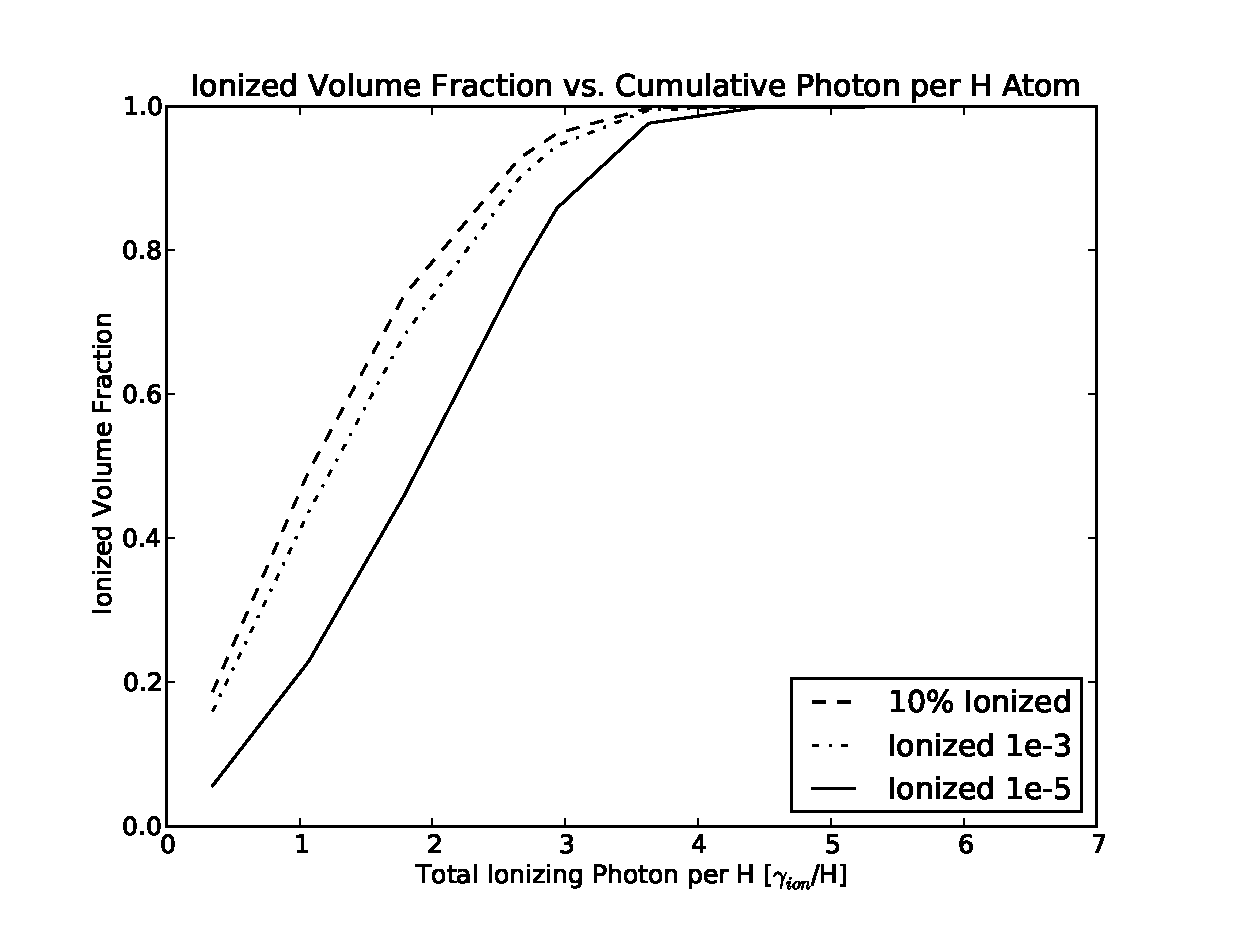
\includegraphics[width=0.5\textwidth]{bnumPhoton_Ion.eps}
  \caption{\footnotesize This graph shows that different amounts of photons is required for different degrees of ionization for a given volume fraction.  This clearly shows that more photons is required for more ionization.}
  \label{numPhoton_Ion}
\end{figure}